\section*{Цель}

Исследование характеристик процесса чистого рождения.

\section*{Порядок выполнения}

\begin{enumerate}
    \item Разработать программу для моделирования процесса чистого рождения. На экран выводить диаграмму состояний процесса и графики значений вероятностей первых одиннадцати состояний, математического ожидания и дисперсии процесса.
    \item Исследовать поведение процесса при заданных последовательностях параметров { $\lambda_k$ }.
    \item Описать поведение процесса при заданных последовательностях параметров { $\lambda_k$ }.
\end{enumerate}

\section*{Исходные данные}

Задана последовательности параметров \{ $\lambda_k$ \}, соответствующие трем моделям процесса чистого рождения.

\begin{align*}
    \lambda_k & = 0.95\\
    \lambda_k & = 0.15k^2 + 4\\
    \lambda_k & = 6.25 / (k+5)
\end{align*}

\section*{Диаграммы состояний}

Для каждой из моделей были построены диаграммы состояний процесса для предварительных прогонов каждой из моделей.

\begin{figure}[h!]
    \centering
    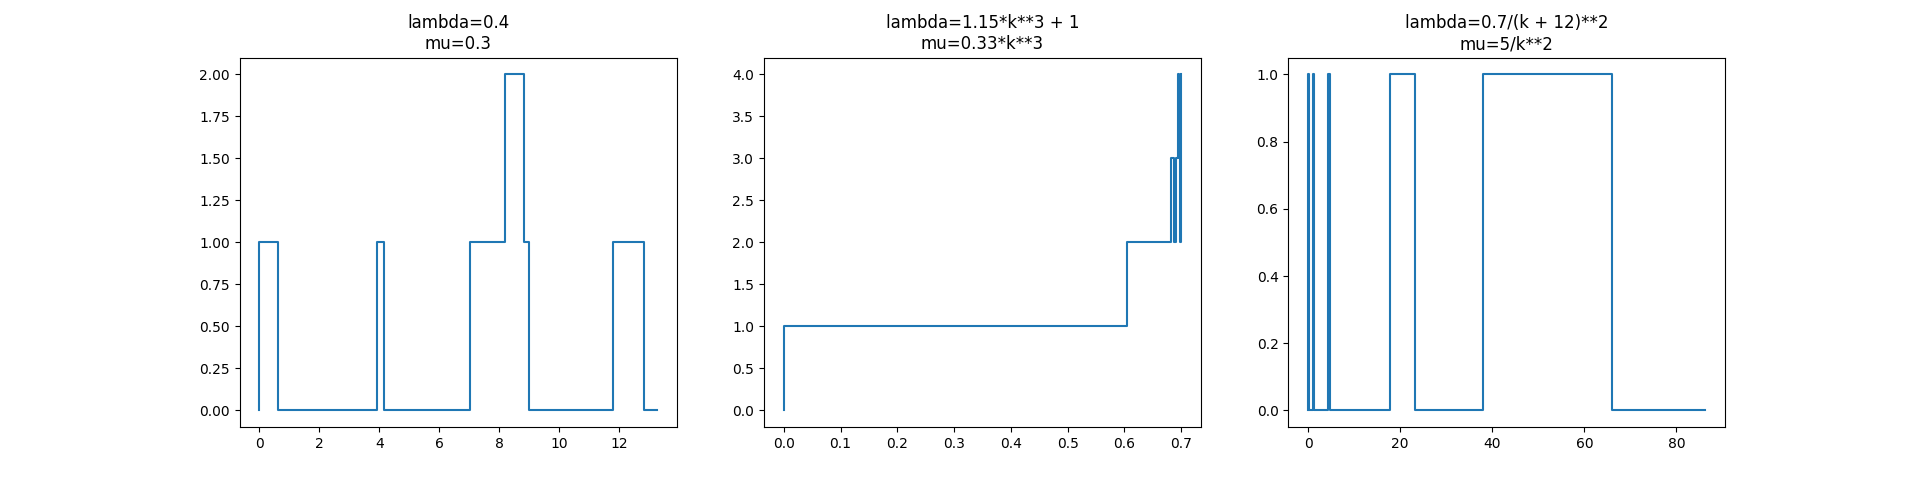
\includegraphics[width=\textwidth]{\jobname/docs/img/state_diagrams.png}
    \caption{Диграммы состояний процесса предварительных прогонов каждой модели}
\end{figure}

\section*{Модель $\lambda_k = 0.95$}

В качестве исследования заданной модели были произведены 200 экспериментов с целью определения вероятностей каждого
из состояний в каждый момент времени $P(X(t)=n)$, а также значений математического ожидания $M(X)$ и дисперсии $D(X)$.
Полученные графики вероятностей, математического ожидания и дисперсии приведены на графиках ниже.

\begin{figure}[h!]
    \centering
    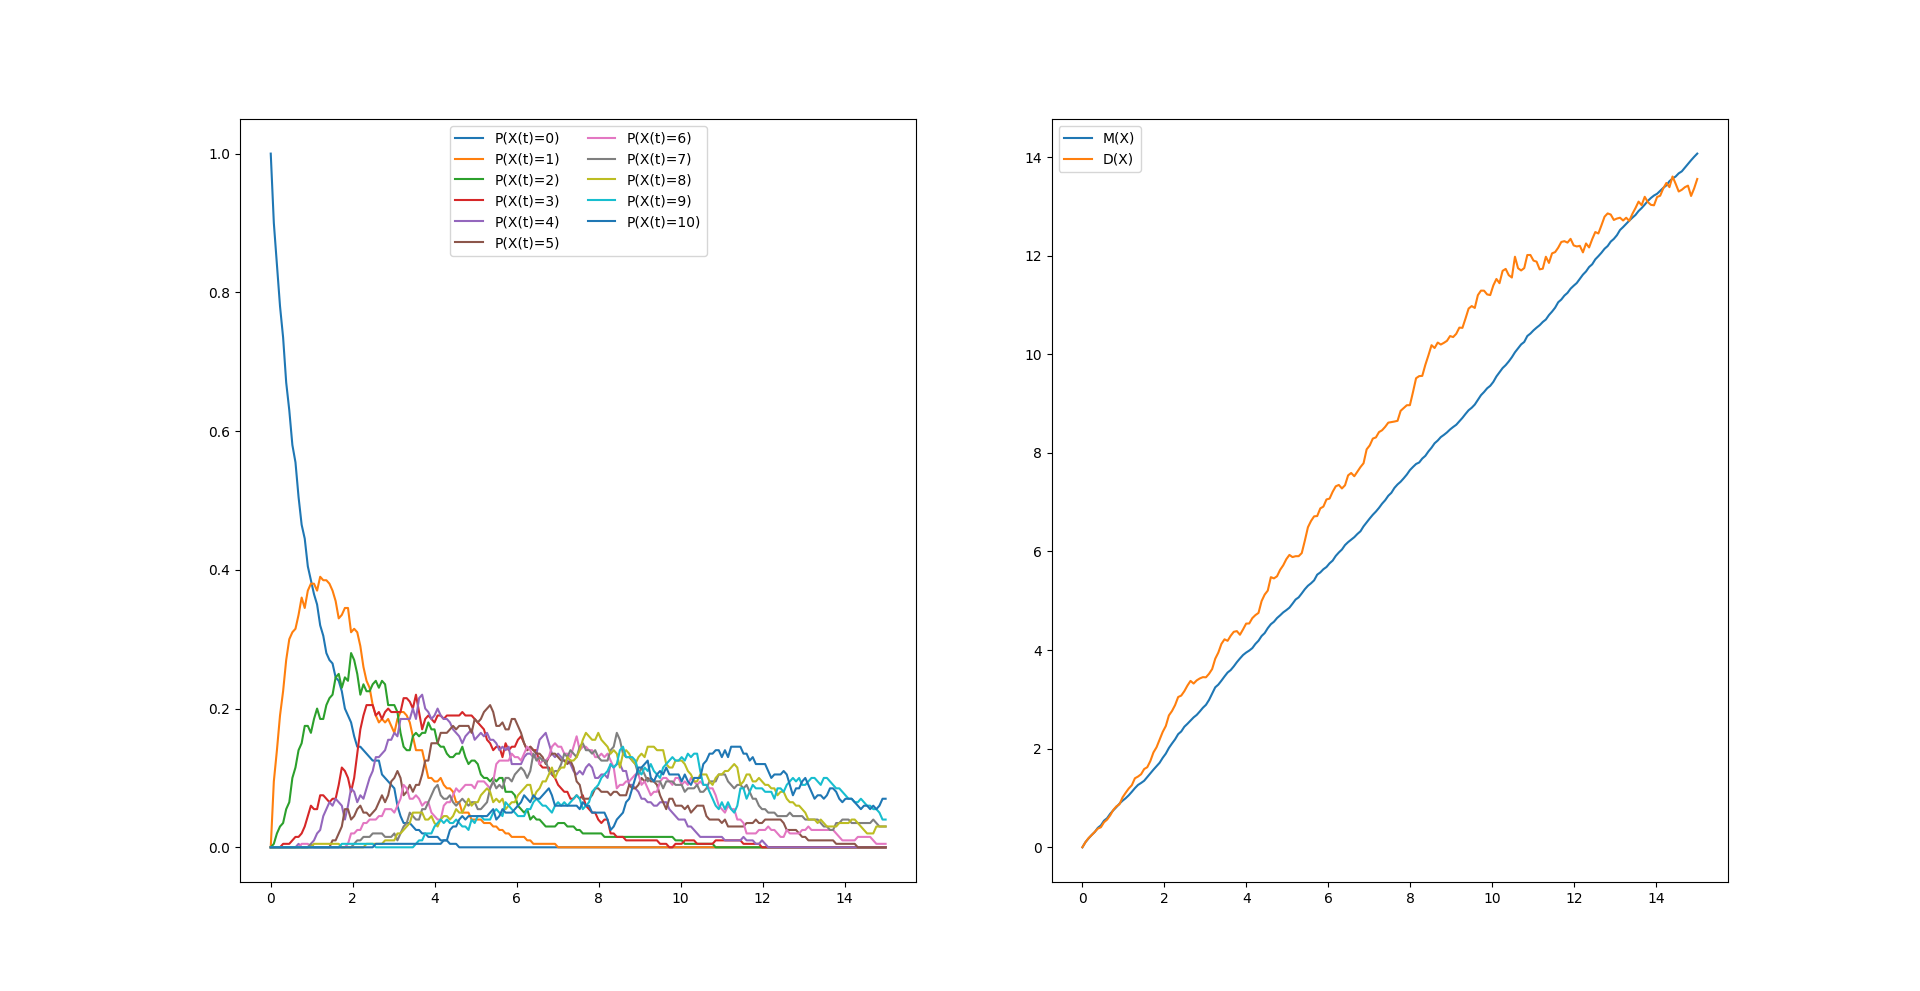
\includegraphics[width=\textwidth]{\jobname/docs/img/model_1.png}
    \caption{Графики вероятностей состояний, математического ожидания и дисперсии при $\lambda_k = 0.95$}
\end{figure}

\section*{Модель $\lambda_k = 0.15k^2 + 4$}

В качестве исследования заданной модели были произведены 200 экспериментов с целью определения вероятностей каждого
из состояний в каждый момент времени $P(X(t)=n)$, а также значений математического ожидания $M(X)$ и дисперсии $D(X)$.
Полученные графики вероятностей, математического ожидания и дисперсии приведены на графиках ниже.

\begin{figure}[h!]
    \centering
    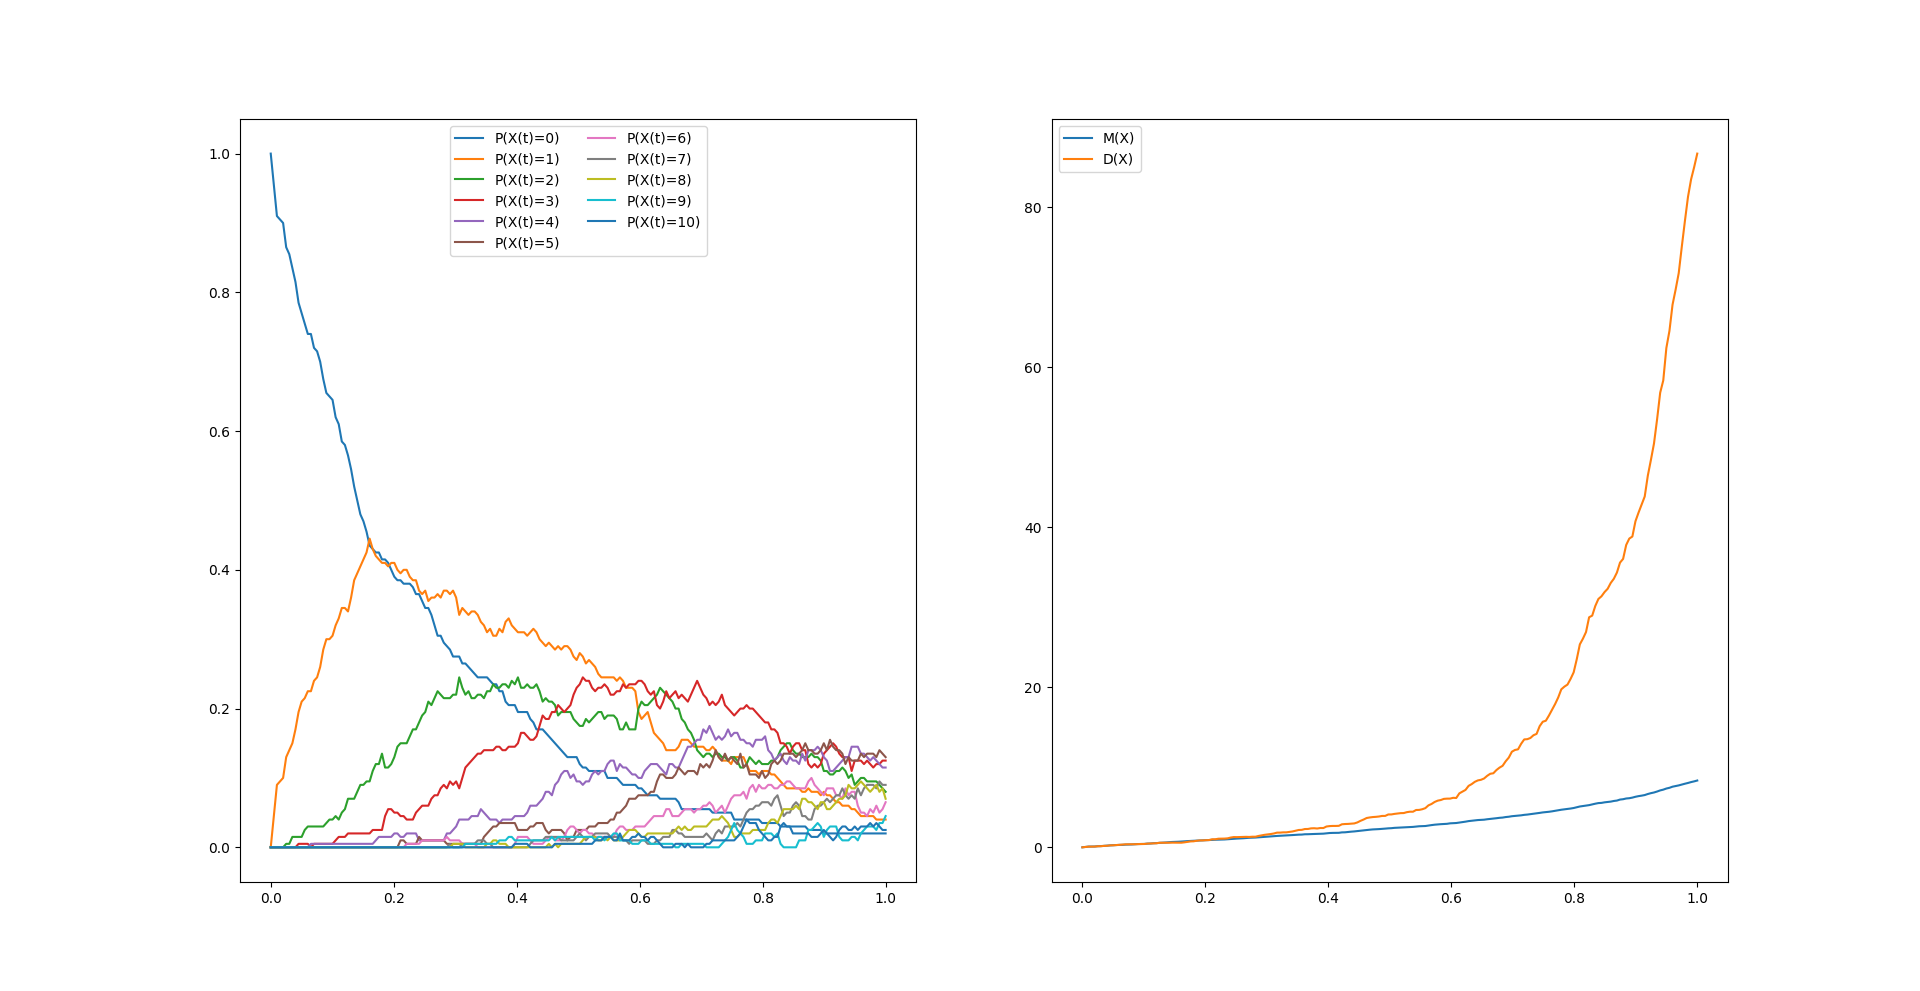
\includegraphics[width=\textwidth]{\jobname/docs/img/model_2.png}
    \caption{Графики вероятностей состояний, математического ожидания и дисперсии при $\lambda_k = 0.15k^2 + 4$}
\end{figure}

\section*{Модель $\lambda_k = 6.25 / (k+5)$}

В качестве исследования заданной модели были произведены 200 экспериментов с целью определения вероятностей каждого
из состояний в каждый момент времени $P(X(t)=n)$, а также значений математического ожидания $M(X)$ и дисперсии $D(X)$.
Полученные графики вероятностей, математического ожидания и дисперсии приведены на графиках ниже.

\begin{figure}[h!]
    \centering
    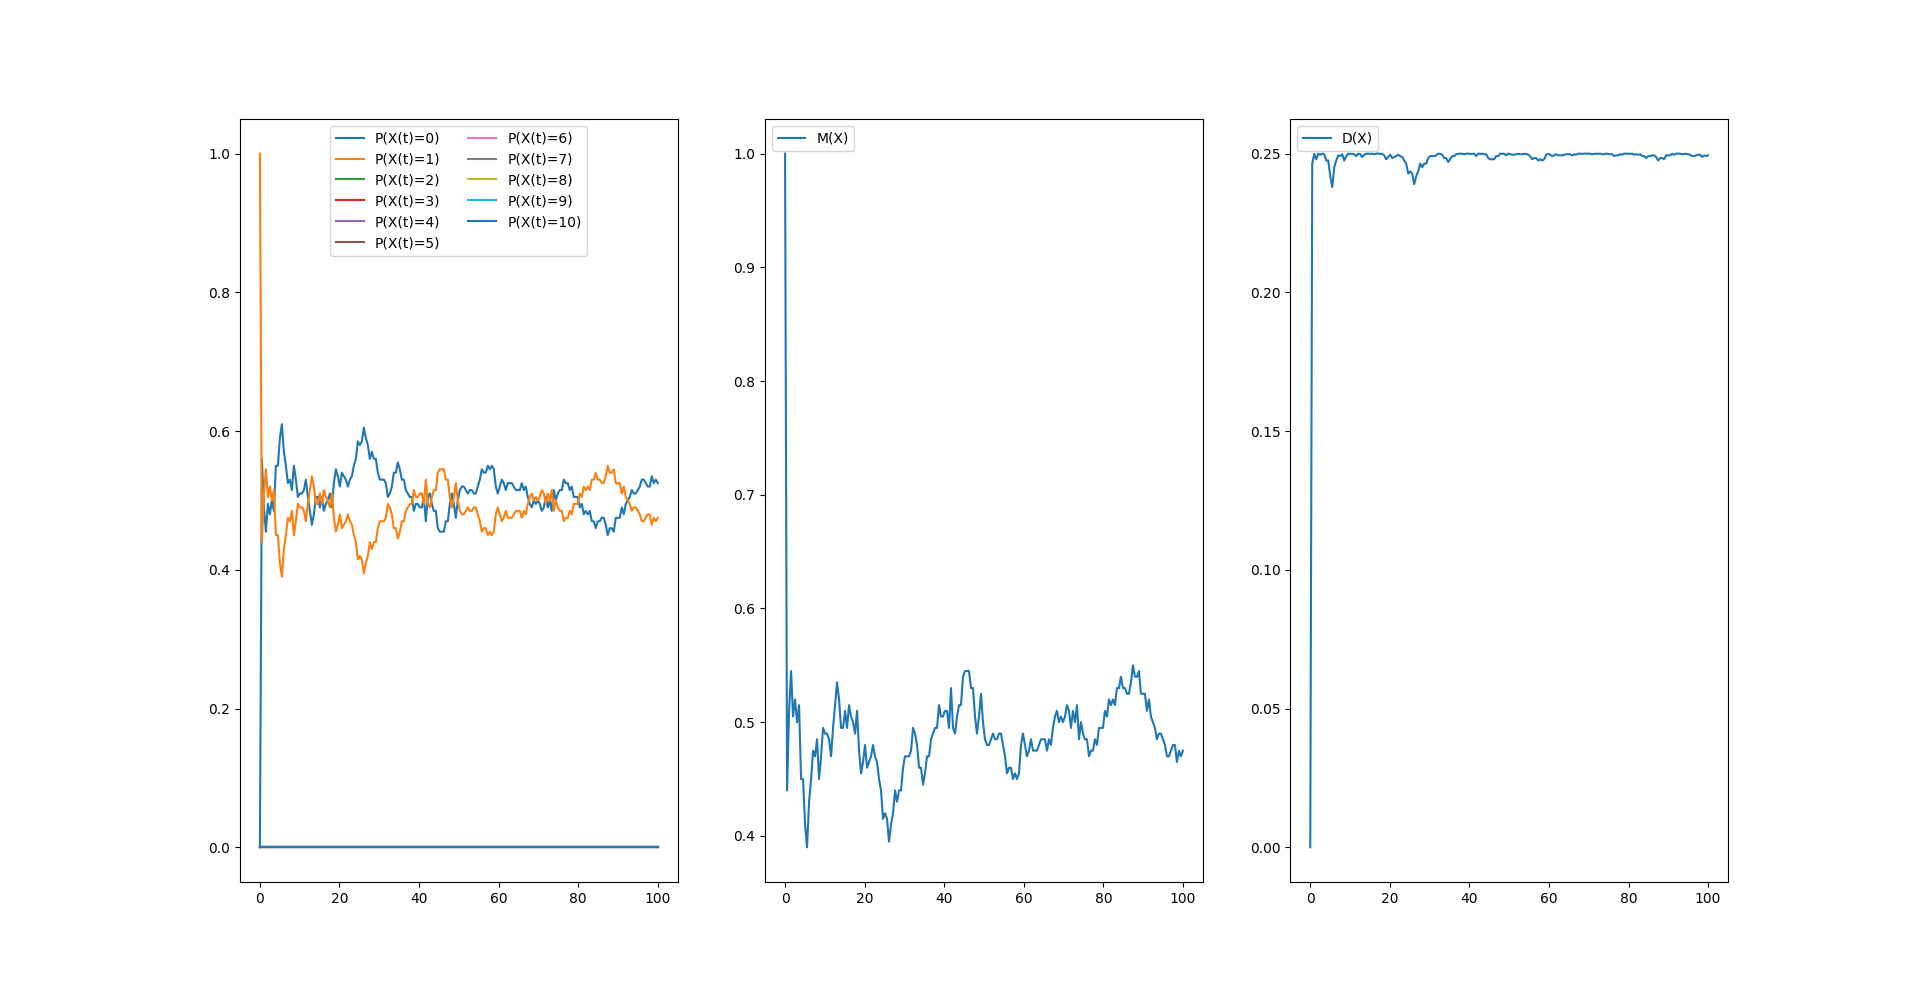
\includegraphics[width=\textwidth]{\jobname/docs/img/model_3.png}
    \caption{Графики вероятностей состояний, математического ожидания и дисперсии при $\lambda_k = 6.25 / (k+5)$}
\end{figure}

\section*{Выводы}

В ходе выполнения лабораторной работы были исследованы три процесса чистого рождения, заданные последовательностями
параметров \{ $\lambda_k$ \}.
Для каждой из моделей были построены диаграммы состояний, графики вероятности случайной величины, математического
ожидания и дисперсии в каждый момент времени.
На основе параметров моделей были составлены характеристики каждого из процессов, описанные ниже.

\subsection*{Первая модель}

В связи с независимостью $\lambda_n$ от текущего состояния, время поступления новых событий не меняется с течением временем.
Можно наблюдать, что математическое ожидание и дисперсия растут практически линейно, что согласуется с предыдущим
утверждением о постоянстве времени поступления новых событий.

\subsection*{Вторая модель}

Во втором случае $\lambda_n$ зависит от квадрата значения текущего состояния, что обеспечивает уменьшение времени поступления
заявок с течением времени.
Можно наблюдать, что скорости роста математического ожидания и дисперсии со временем увеличиваются, что согласуется с
предыдущим утверждением об уменьшении времени поступления новых событий.

\subsection*{Третья модель}

В последней модели $\lambda_n$ обратно зависит от значения текущего состояния, что обеспечивает увеличение времени поступления
заявок с течением времени.
Можно наблюдать, что скорость роста математического ожидания и дисперсии со временем уменьшаются, что согласуется с
предыдущим утверждением об увеличении времени поступления новых событий.

\section*{Листинги}

\subsection*{Листинг основного скрипта}
\lstinputlisting[language=Python,texcl=true]{\jobname/lab.py}

\subsection*{Листинг скрипта, содержащего модель чистого рождения}
\lstinputlisting[language=Python,texcl=true]{\jobname/birth.py}

\subsection*{Листинг скрипта, содержащего генераторы}
\lstinputlisting[language=Python,texcl=true]{\jobname/../common/gen.py}

\subsection*{Листинг скрипта, содержащего утилиты}
\lstinputlisting[language=Python,texcl=true]{\jobname/../common/utils.py}

\subsection*{Листинг скрипта, инициализируещего логирование}
\lstinputlisting[language=Python,texcl=true]{\jobname/../common/log.py}
